\begin{itemize}
  \item IRIS is a framework that addresses the problem of offline policy learning from a large set of diverse and suboptimal demonstrations
  \item Use demonstrated data in lieu of reward function, avoids the problem of exploration
  \item Conventional IL methods assume that demonstration data is near-optimal and unimodal
  \item High-level controller selects a new goal state $s_{g}$ for $T$ timesteps, low-level controller is conditioned on $s_{g}$ and tries to reach that state in the $T$ timesteps
  \item High-level controller has two parts
  \begin{itemize}
    \item conditional VAE (cVAE): predicts the distribution of states $p(s_{t+T}|s_{t})$, used to sample goal proposals
    \item value function $V(s)$ used to select the most promising goal proposal
    \item value function is trained using a simple variant of BCQ
  \end{itemize}
  \item Low-level controller:
  \begin{itemize}
    \item a goal-conditioned RNN that outputs an action $a_{t}$ given $s_{t}$ and $s_{g}$
    \item trained on trajectory sequences from dataset, the last observation in each sequence is treated as the goal
    \item trained using a simple Behavioral Cloning loss
    \item learns to copy action sequence that resulted in a particular observation
  \end{itemize}
  \item This induces \textit{selective imitation}
  \item Experiments:
  \begin{itemize}
    \item Graph reach is 2D navigation domain, contains 250 demonstrations, demonstration paths can take detours
    \item Robosuite Lift: actuate Sawyer robot to grasp and lift cube from table
    \item RoboTurk Can Pick and Place task and Can Image task
    \begin{figure}[h]
      \caption{Tasks}
      \centering
      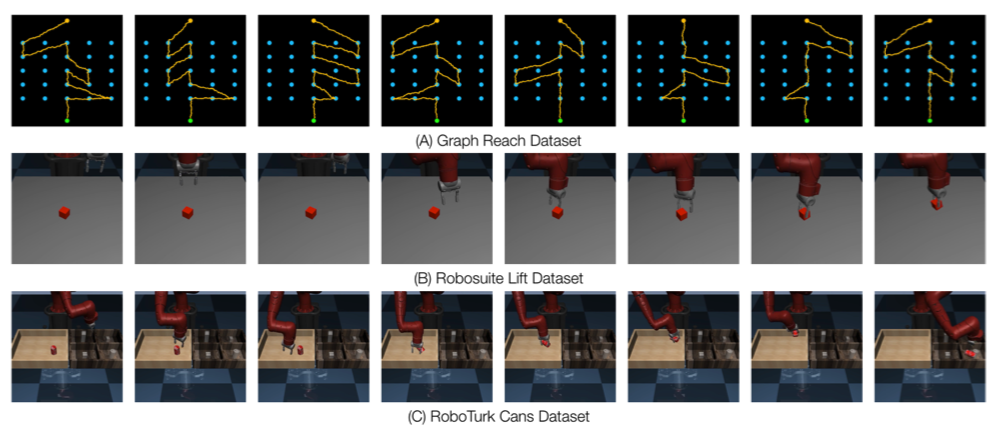
\includegraphics[width=\textwidth]{../../imgs/iris.png}
    \end{figure}
    \item Baselines: BC, BC-RNN, BCQ, IRIS w/o cVAE, IRIS w/o Value Network
    \item All baselines achieve perfect performance on Graph Reach, IRIS 81.3\% on Lift, and 28.3\% on Cans dataset
  \end{itemize}

\end{itemize}